% Simple circle figure: triangle ABC with midline chord GF of circumcircle, CF || AB.
% No extra TikZ libraries required beyond wrapper.
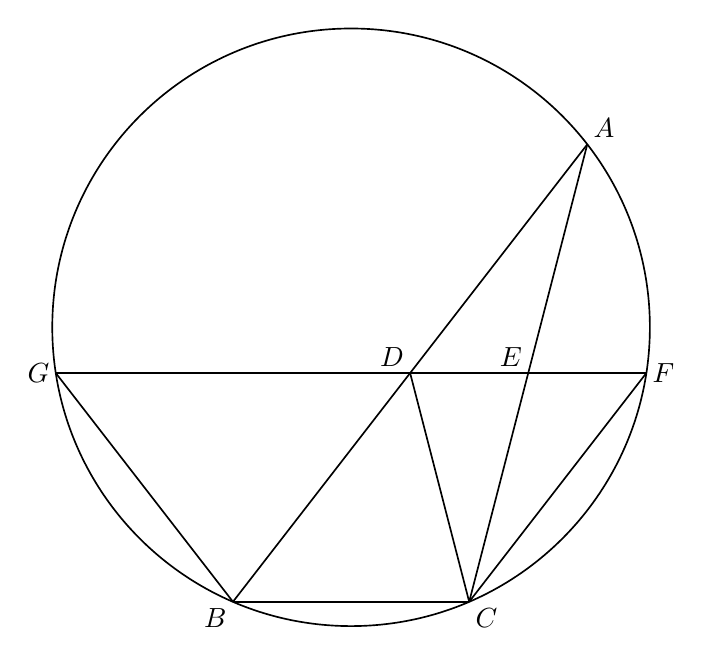
\begin{tikzpicture}[x=1cm,y=1cm,line width=.6pt,font=\normalsize]
\coordinate (O) at (1.5,3.485685);
\coordinate (B) at (0.0,0.0);
\coordinate (C) at (3.0,0.0);
\coordinate (A) at (4.5,5.809475);
\coordinate (G) at (-2.25,2.904738);
\coordinate (D) at (2.25,2.904738);
\coordinate (E) at (3.75,2.904738);
\coordinate (F) at (5.25,2.904738);
\draw (O) circle [radius=3.794733cm];
\draw (G)--(F);
\draw (G)--(B);
\draw (B)--(C);
\draw (C)--(F);
\draw (A)--(B);
\draw (A)--(C);
\draw (D)--(C);
\node[below left=2pt,inner sep=0pt] at (B) {$B$};
\node[below right=2pt,inner sep=0pt] at (C) {$C$};
\node[above right=2pt,inner sep=0pt] at (A) {$A$};
\node[left=2pt,inner sep=0pt] at (G) {$G$};
\node[right=2pt,inner sep=0pt] at (F) {$F$};
\node[above left=2pt,inner sep=0pt] at (D) {$D$};
\node[above left=2pt,inner sep=0pt] at (E) {$E$};
\end{tikzpicture}
